\documentclass[]{article}
\usepackage{lmodern}
\usepackage{amssymb,amsmath}
\usepackage{ifxetex,ifluatex}
\usepackage{fixltx2e} % provides \textsubscript
\ifnum 0\ifxetex 1\fi\ifluatex 1\fi=0 % if pdftex
  \usepackage[T1]{fontenc}
  \usepackage[utf8]{inputenc}
\else % if luatex or xelatex
  \ifxetex
    \usepackage{mathspec}
  \else
    \usepackage{fontspec}
  \fi
  \defaultfontfeatures{Ligatures=TeX,Scale=MatchLowercase}
\fi
% use upquote if available, for straight quotes in verbatim environments
\IfFileExists{upquote.sty}{\usepackage{upquote}}{}
% use microtype if available
\IfFileExists{microtype.sty}{%
\usepackage[]{microtype}
\UseMicrotypeSet[protrusion]{basicmath} % disable protrusion for tt fonts
}{}
\PassOptionsToPackage{hyphens}{url} % url is loaded by hyperref
\usepackage[unicode=true]{hyperref}
\hypersetup{
            pdfborder={0 0 0},
            breaklinks=true}
\urlstyle{same}  % don't use monospace font for urls
\usepackage[margin=1in]{geometry}
\usepackage{color}
\usepackage{fancyvrb}
\newcommand{\VerbBar}{|}
\newcommand{\VERB}{\Verb[commandchars=\\\{\}]}
\DefineVerbatimEnvironment{Highlighting}{Verbatim}{commandchars=\\\{\}}
% Add ',fontsize=\small' for more characters per line
\usepackage{framed}
\definecolor{shadecolor}{RGB}{248,248,248}
\newenvironment{Shaded}{\begin{snugshade}}{\end{snugshade}}
\newcommand{\KeywordTok}[1]{\textcolor[rgb]{0.13,0.29,0.53}{\textbf{#1}}}
\newcommand{\DataTypeTok}[1]{\textcolor[rgb]{0.13,0.29,0.53}{#1}}
\newcommand{\DecValTok}[1]{\textcolor[rgb]{0.00,0.00,0.81}{#1}}
\newcommand{\BaseNTok}[1]{\textcolor[rgb]{0.00,0.00,0.81}{#1}}
\newcommand{\FloatTok}[1]{\textcolor[rgb]{0.00,0.00,0.81}{#1}}
\newcommand{\ConstantTok}[1]{\textcolor[rgb]{0.00,0.00,0.00}{#1}}
\newcommand{\CharTok}[1]{\textcolor[rgb]{0.31,0.60,0.02}{#1}}
\newcommand{\SpecialCharTok}[1]{\textcolor[rgb]{0.00,0.00,0.00}{#1}}
\newcommand{\StringTok}[1]{\textcolor[rgb]{0.31,0.60,0.02}{#1}}
\newcommand{\VerbatimStringTok}[1]{\textcolor[rgb]{0.31,0.60,0.02}{#1}}
\newcommand{\SpecialStringTok}[1]{\textcolor[rgb]{0.31,0.60,0.02}{#1}}
\newcommand{\ImportTok}[1]{#1}
\newcommand{\CommentTok}[1]{\textcolor[rgb]{0.56,0.35,0.01}{\textit{#1}}}
\newcommand{\DocumentationTok}[1]{\textcolor[rgb]{0.56,0.35,0.01}{\textbf{\textit{#1}}}}
\newcommand{\AnnotationTok}[1]{\textcolor[rgb]{0.56,0.35,0.01}{\textbf{\textit{#1}}}}
\newcommand{\CommentVarTok}[1]{\textcolor[rgb]{0.56,0.35,0.01}{\textbf{\textit{#1}}}}
\newcommand{\OtherTok}[1]{\textcolor[rgb]{0.56,0.35,0.01}{#1}}
\newcommand{\FunctionTok}[1]{\textcolor[rgb]{0.00,0.00,0.00}{#1}}
\newcommand{\VariableTok}[1]{\textcolor[rgb]{0.00,0.00,0.00}{#1}}
\newcommand{\ControlFlowTok}[1]{\textcolor[rgb]{0.13,0.29,0.53}{\textbf{#1}}}
\newcommand{\OperatorTok}[1]{\textcolor[rgb]{0.81,0.36,0.00}{\textbf{#1}}}
\newcommand{\BuiltInTok}[1]{#1}
\newcommand{\ExtensionTok}[1]{#1}
\newcommand{\PreprocessorTok}[1]{\textcolor[rgb]{0.56,0.35,0.01}{\textit{#1}}}
\newcommand{\AttributeTok}[1]{\textcolor[rgb]{0.77,0.63,0.00}{#1}}
\newcommand{\RegionMarkerTok}[1]{#1}
\newcommand{\InformationTok}[1]{\textcolor[rgb]{0.56,0.35,0.01}{\textbf{\textit{#1}}}}
\newcommand{\WarningTok}[1]{\textcolor[rgb]{0.56,0.35,0.01}{\textbf{\textit{#1}}}}
\newcommand{\AlertTok}[1]{\textcolor[rgb]{0.94,0.16,0.16}{#1}}
\newcommand{\ErrorTok}[1]{\textcolor[rgb]{0.64,0.00,0.00}{\textbf{#1}}}
\newcommand{\NormalTok}[1]{#1}
\usepackage{graphicx,grffile}
\makeatletter
\def\maxwidth{\ifdim\Gin@nat@width>\linewidth\linewidth\else\Gin@nat@width\fi}
\def\maxheight{\ifdim\Gin@nat@height>\textheight\textheight\else\Gin@nat@height\fi}
\makeatother
% Scale images if necessary, so that they will not overflow the page
% margins by default, and it is still possible to overwrite the defaults
% using explicit options in \includegraphics[width, height, ...]{}
\setkeys{Gin}{width=\maxwidth,height=\maxheight,keepaspectratio}
\IfFileExists{parskip.sty}{%
\usepackage{parskip}
}{% else
\setlength{\parindent}{0pt}
\setlength{\parskip}{6pt plus 2pt minus 1pt}
}
\setlength{\emergencystretch}{3em}  % prevent overfull lines
\providecommand{\tightlist}{%
  \setlength{\itemsep}{0pt}\setlength{\parskip}{0pt}}
\setcounter{secnumdepth}{0}
% Redefines (sub)paragraphs to behave more like sections
\ifx\paragraph\undefined\else
\let\oldparagraph\paragraph
\renewcommand{\paragraph}[1]{\oldparagraph{#1}\mbox{}}
\fi
\ifx\subparagraph\undefined\else
\let\oldsubparagraph\subparagraph
\renewcommand{\subparagraph}[1]{\oldsubparagraph{#1}\mbox{}}
\fi

% set default figure placement to htbp
\makeatletter
\def\fps@figure{htbp}
\makeatother


\author{}
\date{\vspace{-2.5em}}

\begin{document}

\section{Les données vectorielles}\label{vec}

L'objectif principal de ce module est d'apprendre à lire, interpréter et
visualiser des données vectorielles.

À la fin de ce module vous saurez:

\begin{itemize}
\tightlist
\item
  Lire un shapefile, explorer ses métadonnées et interpréter sa
  géométrie
\item
  Visualiser des données vectorielles de type point, ligne et polygone
\item
  Visualiser des données vectorielles par attribut
\item
  Visualiser plusieurs données vectorielles au sein d'une même figure
\item
  Transformer le système de coordonnées de référence de données
  vectorielles
\end{itemize}

Vous utiliserez les librairies suivantes:

\begin{itemize}
\tightlist
\item
  \texttt{sf}
\item
  \texttt{rgdal}
\item
  \texttt{dplyr}
\item
  \texttt{ggplot2}
\item
  \texttt{ggpubr}
\end{itemize}

Vous apprendrez à utiliser les fonctions suivantes:

\begin{itemize}
\tightlist
\item
  \texttt{st\_read()}, \texttt{st\_write()}
\item
  \texttt{st\_geometry\_type()}
\item
  \texttt{st\_crs()}
\item
  \texttt{st\_bbox()}
\item
  \texttt{geom\_sf}
\item
  \texttt{filter()}
\item
  \texttt{st\_transform()}
\item
  \texttt{ggarrange()}
\end{itemize}

Dans la section Leçon, vous utiliserez des données vectorielles
relatives au réseau de pistes cyclables de la ville de Montréal et aux
accidents routiers impliquant des bicyclettes. Ces données sont
disponibles
\href{https://github.com/elisefilotas/Donnees_spatiales/blob/master/Montreal_Velo.zip}{ici}.

Dans la section Exercice, vous utiliserez XXXXX

\subsection{Leçon}\label{leuxe7on}

L'ensemble du MATERIEL disponible dans ce module est adapté du cours
\emph{Introduction to Geospatial Raster and Vector Data with
R}\footnote{Wasser, L. A., Jones, M. A., Brum, Z., Riemer, K., Williams,
  J., Hollister, J., . . . Stachelek, J. Introduction to Geospatial
  Raster and Vector Data with R. Repéré le 1er mars 2020 à
  \url{https://datacarpentry.org/r-raster-vector-geospatial/}} de
l'organisme \href{https://datacarpentry.org/}{Data Carpentry}. Data
Carpentry développe et offre des formations variées et spécialisées sur
le traitement et l'analyse de données. Ses formations s'adressent
surtout aux chercheuses et chercheurs scientifiques, mais peuvent être
consultées par quiconque car leur matériel est libre d'accès. N'hésitez
donc pas à y jeter un coup d'œil.

Dans le cadre de cette leçon, nous allons explorer des données
vectorielles relatives au réseau de pistes cyclables de la ville de
Montréal et aux accidents routiers impliquant des bicyclettes.
Téléchargez les données en cliquant sur ce
\href{https://github.com/elisefilotas/Donnees_spatiales/blob/master/Montreal_Velo.zip}{lien}.
Sauvegardez le dossier compressé (\texttt{zip}) dans votre répertoire de
travail `Donnees' pour ce module, et dézippez-le. Le dossier
Montreal\_Velo comprend trois sous-dossiers:

\begin{itemize}
\tightlist
\item
  accidents,
\item
  pistes, et
\item
  terre.
\end{itemize}

\subsubsection{Introduction aux données vectorielles sous
R}\label{introduction-aux-donnuxe9es-vectorielles-sous-r}

\paragraph{Lire un shapefile et interpréter sa
géométrie}\label{lire-un-shapefile-et-interpruxe9ter-sa-guxe9omuxe9trie}
\addcontentsline{toc}{paragraph}{Lire un shapefile et interpréter sa
géométrie}

Pour lire des données vectorielles contenues dans un fichier shapefile,
nous allons utiliser la librairie \texttt{sf}. Notez que la librairie
\texttt{rgdal} se charge automatiquement lorsque \texttt{sf} se charge.

\begin{Shaded}
\begin{Highlighting}[]
\KeywordTok{library}\NormalTok{(sf)}
\end{Highlighting}
\end{Shaded}

Les shapefiles que nous allons lire sont les suivants :

\begin{itemize}
\tightlist
\item
  Des données vectorielles de type polygone représentant la frontière de
  notre zone d'étude, ici, l'île de Montréal.
\item
  Des données vectorielles de type ligne représentant les pistes
  cyclables sur l'île de Montréal, et
\item
  Des données vectorielles de type point représentant la position
  d'accidents impliquant des bicyclettes.
\end{itemize}

Les premières données vectorielles que nous allons ouvrir contiennent
les limites terrestres de l'île de Montréal. Pour lire ces données nous
utiliserons la fonction \texttt{st\_read()} de la librarie \texttt{sf}.
Pour utiliser \texttt{st\_read()} nous devons spécifier le chemin menant
au fichier shapefile à lire.

\begin{Shaded}
\begin{Highlighting}[]
\NormalTok{chemin<-}\StringTok{"D:/votrechemin/SCI1031/Module3/Donnees/"}
\NormalTok{nom_du_fichier <-}\StringTok{ }\KeywordTok{paste}\NormalTok{(chemin, }\StringTok{"/Montreal_Velo/terre/terre_shp.shp"}\NormalTok{, }\DataTypeTok{sep =} \StringTok{""}\NormalTok{)}
\NormalTok{limites_terrestres <-}\StringTok{ }\KeywordTok{st_read}\NormalTok{(nom_du_fichier)}
\end{Highlighting}
\end{Shaded}

\begin{verbatim}
## Reading layer `terre_shp' from data source `E:\ELF\Dropbox\Teluq\Enseignement\Cours\AnalyseSpatiale\Developpement\Structure_test\sci1031\Module3\data\Montreal_Velo\terre\terre_shp.shp' using driver `ESRI Shapefile'
## Simple feature collection with 72 features and 1 field
## geometry type:  POLYGON
## dimension:      XY
## bbox:           xmin: 267517.3 ymin: 5029232 xmax: 306669.4 ymax: 5062642
## epsg (SRID):    NA
## proj4string:    +proj=tmerc +lat_0=0 +lon_0=-73.5 +k=0.9999 +x_0=304800 +y_0=0 +datum=NAD83 +units=m +no_defs
\end{verbatim}

La fonction \texttt{st\_read()} vous permet d'ores et déjà d'obtenir
certaines informations sur la structure des données vectorielles que
vous venez de lire: le type de géométrie (\texttt{geometry\ type}), la
dimension des données (\texttt{dimension}), l'étendue spatiale des
données (\texttt{bbox}), et les informations relatives au système de
coordonnées de référence, le SPSG (\texttt{epsg\ (SRID)}) et la
projection (\texttt{proj4string}). Nous explorerons ces propriétés en
détails plus bas.

Nous allons maintenant lire les données vectorielles de type ligne, en
utilisant encore la fonction \texttt{st\_read()}.

\texttt{r\ chemin\ \textless{}-"D:/votrechemin/SCI1031/Module3/Donnees/"\ nom\_du\_fichier\textless{}-\ paste(chemin,\ "/Montreal\_Velo/pistes/pistes\_cyclables\_type.shp",\ sep\ =\ "")\ pistes\_cyclables\ \textless{}-\ st\_read(nom\_du\_fichier)}\#

\begin{verbatim}
\end{verbatim}

\subsection{\texorpdfstring{Reading layer
\texttt{LIMADMIN\textquotesingle{}\ from\ data\ source}E:\ELF\Dropbox\Teluq\Enseignement\Cours\AnalyseSpatiale\Developpement\Structure\_test\sci1031\Module3\data\LIMADMIN.shp'
using driver `ESRI Shapefile' \#\# Simple feature collection with 34
features and 9 fields \#\# geometry type: MULTIPOLYGON \#\# dimension:
XY \#\# bbox: xmin: -73.9966 ymin: 45.3854 xmax: -73.47387 ymax:
45.70758 \#\# epsg (SRID): 4326 \#\# proj4string: +proj=longlat
+datum=WGS84 +no\_defs
```}{Reading layer LIMADMIN' from data sourceE:\_test10313.shp' using driver `ESRI Shapefile' \#\# Simple feature collection with 34 features and 9 fields \#\# geometry type: MULTIPOLYGON \#\# dimension: XY \#\# bbox: xmin: -73.9966 ymin: 45.3854 xmax: -73.47387 ymax: 45.70758 \#\# epsg (SRID): 4326 \#\# proj4string: +proj=longlat +datum=WGS84 +no\_defs ```}}\label{reading-layer-limadmin-from-data-sourcee_test10313.shp-using-driver-esri-shapefile-simple-feature-collection-with-34-features-and-9-fields-geometry-type-multipolygon-dimension-xy-bbox-xmin--73.9966-ymin-45.3854-xmax--73.47387-ymax-45.70758-epsg-srid-4326-proj4string-projlonglat-datumwgs84-no_defs}

Finalement, nous allons lire les données vectorielles de type point, en
utilisant toujours la fonction \texttt{st\_read()}.

\begin{Shaded}
\begin{Highlighting}[]
\NormalTok{chemin<-}\StringTok{"D:/votrechemin/SCI1031/Module3/Donnees/"}
\NormalTok{nom_du_fichier<-}\StringTok{ }\KeywordTok{paste}\NormalTok{(chemin, }\StringTok{"/Montreal_Velo/accidents/accidents2018_Mtl_velo.shp"}\NormalTok{, }\DataTypeTok{sep =} \StringTok{""}\NormalTok{)}
\NormalTok{pistes_cyclables <-}\StringTok{ }\KeywordTok{st_read}\NormalTok{(nom_du_fichier)}
\end{Highlighting}
\end{Shaded}

\begin{Shaded}
\begin{Highlighting}[]
\CommentTok{# nom_du_fichier<- paste(module, "/Montreal_Velo/accidents/accidents2018_Mtl_velo.shp", sep = "")}
\CommentTok{# accidents_velo <- st_read(nom_du_fichier)}
\NormalTok{accidents_velo <-}\StringTok{ }\KeywordTok{st_read}\NormalTok{(}\StringTok{"Module3/data/LIMADMIN.shp"}\NormalTok{)}
\end{Highlighting}
\end{Shaded}

\begin{verbatim}
## Reading layer `LIMADMIN' from data source `E:\ELF\Dropbox\Teluq\Enseignement\Cours\AnalyseSpatiale\Developpement\Structure_test\sci1031\Module3\data\LIMADMIN.shp' using driver `ESRI Shapefile'
## Simple feature collection with 34 features and 9 fields
## geometry type:  MULTIPOLYGON
## dimension:      XY
## bbox:           xmin: -73.9966 ymin: 45.3854 xmax: -73.47387 ymax: 45.70758
## epsg (SRID):    4326
## proj4string:    +proj=longlat +datum=WGS84 +no_defs
\end{verbatim}

Remarquez que le type de géométrie (\texttt{geometry\ type}) diffère
pour les trois classes de données lues.

\paragraph{Explorer les métadonnées d'un
shapefile}\label{explorer-les-muxe9tadonnuxe9es-dun-shapefile}
\addcontentsline{toc}{paragraph}{Explorer les métadonnées d'un
shapefile}

Les informations contenues dans un shapefile sont appelées des
métadonnées. Nous sommes particulièrement intéressées aux métadonnées
géospatiales.

Les métadonnées fondamentales d'un shapefile sont :

\begin{enumerate}
\def\labelenumi{\arabic{enumi}.}
\tightlist
\item
  Type de géométrie : le type de classes des données vectorielles
  téléchargées.
\item
  La projection : le système de coordonnées de référence utilisé pour
  représenter les données.
\item
  L'étendue spatiale : la superficie géographique couvrant les données
  vectorielles.
\end{enumerate}

Nous pouvons explorer chacune de ces métadonnées en utilisant des
fonctions de la librairie \texttt{sf}. Le type de géométrie est obtenu
par la fonction \texttt{st\_geometry\_type()}. Par exemple, pour les
limites terrestres de la ville de Montréal, nous avons :

\begin{Shaded}
\begin{Highlighting}[]
\KeywordTok{st_geometry_type}\NormalTok{(limites_terrestres)}
\end{Highlighting}
\end{Shaded}

\begin{verbatim}
##  [1] POLYGON POLYGON POLYGON POLYGON POLYGON POLYGON POLYGON POLYGON POLYGON
## [10] POLYGON POLYGON POLYGON POLYGON POLYGON POLYGON POLYGON POLYGON POLYGON
## [19] POLYGON POLYGON POLYGON POLYGON POLYGON POLYGON POLYGON POLYGON POLYGON
## [28] POLYGON POLYGON POLYGON POLYGON POLYGON POLYGON POLYGON POLYGON POLYGON
## [37] POLYGON POLYGON POLYGON POLYGON POLYGON POLYGON POLYGON POLYGON POLYGON
## [46] POLYGON POLYGON POLYGON POLYGON POLYGON POLYGON POLYGON POLYGON POLYGON
## [55] POLYGON POLYGON POLYGON POLYGON POLYGON POLYGON POLYGON POLYGON POLYGON
## [64] POLYGON POLYGON POLYGON POLYGON POLYGON POLYGON POLYGON POLYGON POLYGON
## 18 Levels: GEOMETRY POINT LINESTRING POLYGON MULTIPOINT ... TRIANGLE
\end{verbatim}

Nous avons ainsi la confirmation que ces données vectorielles
correspondent des polygones (plus exactement, 72 polygones). Les 18
niveaux donnés en dessous constituent une liste des classes possibles de
géométrie.

En comparaison, pour les données de type ligne et de type point nous
obtenons plutôt :

\begin{Shaded}
\begin{Highlighting}[]
\KeywordTok{st_geometry_type}\NormalTok{(pistes_cyclables)}
\end{Highlighting}
\end{Shaded}

\begin{verbatim}
##  [1] MULTIPOLYGON MULTIPOLYGON MULTIPOLYGON MULTIPOLYGON MULTIPOLYGON
##  [6] MULTIPOLYGON MULTIPOLYGON MULTIPOLYGON MULTIPOLYGON MULTIPOLYGON
## [11] MULTIPOLYGON MULTIPOLYGON MULTIPOLYGON MULTIPOLYGON MULTIPOLYGON
## [16] MULTIPOLYGON MULTIPOLYGON MULTIPOLYGON MULTIPOLYGON MULTIPOLYGON
## [21] MULTIPOLYGON MULTIPOLYGON MULTIPOLYGON MULTIPOLYGON MULTIPOLYGON
## [26] MULTIPOLYGON MULTIPOLYGON MULTIPOLYGON MULTIPOLYGON MULTIPOLYGON
## [31] MULTIPOLYGON MULTIPOLYGON MULTIPOLYGON MULTIPOLYGON
## 18 Levels: GEOMETRY POINT LINESTRING POLYGON MULTIPOINT ... TRIANGLE
\end{verbatim}

\begin{Shaded}
\begin{Highlighting}[]
\KeywordTok{st_geometry_type}\NormalTok{(accidents_velo)}
\end{Highlighting}
\end{Shaded}

\begin{verbatim}
##  [1] MULTIPOLYGON MULTIPOLYGON MULTIPOLYGON MULTIPOLYGON MULTIPOLYGON
##  [6] MULTIPOLYGON MULTIPOLYGON MULTIPOLYGON MULTIPOLYGON MULTIPOLYGON
## [11] MULTIPOLYGON MULTIPOLYGON MULTIPOLYGON MULTIPOLYGON MULTIPOLYGON
## [16] MULTIPOLYGON MULTIPOLYGON MULTIPOLYGON MULTIPOLYGON MULTIPOLYGON
## [21] MULTIPOLYGON MULTIPOLYGON MULTIPOLYGON MULTIPOLYGON MULTIPOLYGON
## [26] MULTIPOLYGON MULTIPOLYGON MULTIPOLYGON MULTIPOLYGON MULTIPOLYGON
## [31] MULTIPOLYGON MULTIPOLYGON MULTIPOLYGON MULTIPOLYGON
## 18 Levels: GEOMETRY POINT LINESTRING POLYGON MULTIPOINT ... TRIANGLE
\end{verbatim}

Vous remarquez alors que les pistes cyclables sont composées de
nombreuses multilignes. Une multiligne étant elle-même un ensemble de
lignes. Quant aux accidents de vélo, on en compte 796 en 2018.

Vérifions maintenant la projection des shapefiles en utilisant la
fonction \texttt{st\_crs()} de la librarie \texttt{sf}:

\begin{Shaded}
\begin{Highlighting}[]
\KeywordTok{st_crs}\NormalTok{(limites_terrestres)}
\end{Highlighting}
\end{Shaded}

\begin{verbatim}
## Coordinate Reference System:
##   No EPSG code
##   proj4string: "+proj=tmerc +lat_0=0 +lon_0=-73.5 +k=0.9999 +x_0=304800 +y_0=0 +datum=NAD83 +units=m +no_defs"
\end{verbatim}

\begin{Shaded}
\begin{Highlighting}[]
\KeywordTok{st_crs}\NormalTok{(pistes_cyclables)}
\end{Highlighting}
\end{Shaded}

\begin{verbatim}
## Coordinate Reference System:
##   EPSG: 4326 
##   proj4string: "+proj=longlat +datum=WGS84 +no_defs"
\end{verbatim}

\begin{Shaded}
\begin{Highlighting}[]
\KeywordTok{st_crs}\NormalTok{(accidents_velo)}
\end{Highlighting}
\end{Shaded}

\begin{verbatim}
## Coordinate Reference System:
##   EPSG: 4326 
##   proj4string: "+proj=longlat +datum=WGS84 +no_defs"
\end{verbatim}

Les données de tous les shapefiles sont dans la projection de Mercator
transverse (\texttt{tmerc}) et utilisent le Système de référence
géodésique nord-américan de 1983 (\texttt{NAD83}). Il n'y a pas de EPSG
assigné à ces données. Connaitre le SCR est essentiel pour interpréter
l'étendue spatiale des objets spatiaux puisque celui-ci précise, en
quelque sorte, les unités de mesure.

Pour connaître l'étendue spatiale des shapefiles, nous utilisons la
fonction \texttt{st\_bbox()} de la librairie \texttt{sf} :

\begin{Shaded}
\begin{Highlighting}[]
\KeywordTok{st_bbox}\NormalTok{(limites_terrestres)}
\end{Highlighting}
\end{Shaded}

\begin{verbatim}
##      xmin      ymin      xmax      ymax 
##  267517.3 5029231.9  306669.4 5062642.4
\end{verbatim}

\begin{Shaded}
\begin{Highlighting}[]
\KeywordTok{st_bbox}\NormalTok{(pistes_cyclables)}
\end{Highlighting}
\end{Shaded}

\begin{verbatim}
##      xmin      ymin      xmax      ymax 
## -73.99660  45.38540 -73.47387  45.70758
\end{verbatim}

\begin{Shaded}
\begin{Highlighting}[]
\KeywordTok{st_bbox}\NormalTok{(accidents_velo)}
\end{Highlighting}
\end{Shaded}

\begin{verbatim}
##      xmin      ymin      xmax      ymax 
## -73.99660  45.38540 -73.47387  45.70758
\end{verbatim}

L'étendue spatiale d'un shapefile ou d'un objet spatial dans \texttt{R}
représente les limites géographiques des données, ou la localisation des
données les plus au sud, nord, est et ouest.

ICI BESOIN D'UNE FIGURE COMME CELLE DE NEON

Finalement, nous pouvons visualiser toutes les métadonnées et les
attributs d'un shapefile simplement en écrivant son nom dans la console
\texttt{R}:

\begin{Shaded}
\begin{Highlighting}[]
\NormalTok{limites_terrestres}
\end{Highlighting}
\end{Shaded}

\begin{verbatim}
## Simple feature collection with 72 features and 1 field
## geometry type:  POLYGON
## dimension:      XY
## bbox:           xmin: 267517.3 ymin: 5029232 xmax: 306669.4 ymax: 5062642
## epsg (SRID):    NA
## proj4string:    +proj=tmerc +lat_0=0 +lon_0=-73.5 +k=0.9999 +x_0=304800 +y_0=0 +datum=NAD83 +units=m +no_defs
## First 10 features:
##    DefaultAtt                       geometry
## 1        <NA> POLYGON ((299607.6 5038364,...
## 2        <NA> POLYGON ((301349.7 5036978,...
## 3        <NA> POLYGON ((300403.5 5038997,...
## 4        <NA> POLYGON ((300743.9 5039496,...
## 5        <NA> POLYGON ((302032.4 5043372,...
## 6        <NA> POLYGON ((302299.3 5043145,...
## 7        <NA> POLYGON ((302508.4 5040978,...
## 8        <NA> POLYGON ((304719.4 5062024,...
## 9        <NA> POLYGON ((304926.9 5062499,...
## 10       <NA> POLYGON ((305395.9 5062622,...
\end{verbatim}

\begin{Shaded}
\begin{Highlighting}[]
\NormalTok{pistes_cyclables}
\end{Highlighting}
\end{Shaded}

\begin{verbatim}
## Simple feature collection with 34 features and 10 fields
## geometry type:  MULTIPOLYGON
## dimension:      XY
## bbox:           xmin: -73.9966 ymin: 45.3854 xmax: -73.47387 ymax: 45.70758
## epsg (SRID):    4326
## proj4string:    +proj=longlat +datum=WGS84 +no_defs
## First 10 features:
##    MUNID CODEID CODEMAMROT                                      NOM
## 1  66023     11      REM05                                Outremont
## 2  66023     22      REM17                                  LaSalle
## 3  66023     62      66072                               Mont-Royal
## 4  66023      9      REM19                              Ville-Marie
## 5  66023      5      REM21                    Le Plateau-Mont-Royal
## 6  66023     54      66062                                Hampstead
## 7  66023     63      REM20                             Le Sud-Ouest
## 8  66023     57      REM33 Rivière-des-Prairies-Pointe-aux-Trembles
## 9  66023     28      REM27                                  Lachine
## 10 66023     51      66087                                   Dorval
##              TYPE ABREV NUM     AIRE     PERIM                       geometry
## 1  Arrondissement    OM   5  3813356 10836.670 MULTIPOLYGON (((-73.62078 4...
## 2  Arrondissement    LS  18 25197268 25259.849 MULTIPOLYGON (((-73.6661 45...
## 3      Ville liée    MR   2  7445560 18314.038 MULTIPOLYGON (((-73.65075 4...
## 4  Arrondissement    VM  20 21500632 26585.959 MULTIPOLYGON (((-73.53013 4...
## 5  Arrondissement    PM  22  8151665 13158.328 MULTIPOLYGON (((-73.55923 4...
## 6      Ville liée    HS  10  1768055  5875.848 MULTIPOLYGON (((-73.65601 4...
## 7  Arrondissement    SO  21 18144269 29633.161 MULTIPOLYGON (((-73.62908 4...
## 8  Arrondissement    RP  19 50047004 38573.067 MULTIPOLYGON (((-73.62475 4...
## 9  Arrondissement    LC  17 23127786 25399.526 MULTIPOLYGON (((-73.72299 4...
## 10     Ville liée    DV   1 28156150 32357.566 MULTIPOLYGON (((-73.7947 45...
##    TYPE_VOIE
## 1          1
## 2          2
## 3          3
## 4          4
## 5          5
## 6          1
## 7          2
## 8          3
## 9          4
## 10         5
\end{verbatim}

\begin{Shaded}
\begin{Highlighting}[]
\NormalTok{accidents_velo}
\end{Highlighting}
\end{Shaded}

\begin{verbatim}
## Simple feature collection with 34 features and 9 fields
## geometry type:  MULTIPOLYGON
## dimension:      XY
## bbox:           xmin: -73.9966 ymin: 45.3854 xmax: -73.47387 ymax: 45.70758
## epsg (SRID):    4326
## proj4string:    +proj=longlat +datum=WGS84 +no_defs
## First 10 features:
##    MUNID CODEID CODEMAMROT                                      NOM
## 1  66023     11      REM05                                Outremont
## 2  66023     22      REM17                                  LaSalle
## 3  66023     62      66072                               Mont-Royal
## 4  66023      9      REM19                              Ville-Marie
## 5  66023      5      REM21                    Le Plateau-Mont-Royal
## 6  66023     54      66062                                Hampstead
## 7  66023     63      REM20                             Le Sud-Ouest
## 8  66023     57      REM33 Rivière-des-Prairies-Pointe-aux-Trembles
## 9  66023     28      REM27                                  Lachine
## 10 66023     51      66087                                   Dorval
##              TYPE ABREV NUM     AIRE     PERIM                       geometry
## 1  Arrondissement    OM   5  3813356 10836.670 MULTIPOLYGON (((-73.62078 4...
## 2  Arrondissement    LS  18 25197268 25259.849 MULTIPOLYGON (((-73.6661 45...
## 3      Ville liée    MR   2  7445560 18314.038 MULTIPOLYGON (((-73.65075 4...
## 4  Arrondissement    VM  20 21500632 26585.959 MULTIPOLYGON (((-73.53013 4...
## 5  Arrondissement    PM  22  8151665 13158.328 MULTIPOLYGON (((-73.55923 4...
## 6      Ville liée    HS  10  1768055  5875.848 MULTIPOLYGON (((-73.65601 4...
## 7  Arrondissement    SO  21 18144269 29633.161 MULTIPOLYGON (((-73.62908 4...
## 8  Arrondissement    RP  19 50047004 38573.067 MULTIPOLYGON (((-73.62475 4...
## 9  Arrondissement    LC  17 23127786 25399.526 MULTIPOLYGON (((-73.72299 4...
## 10     Ville liée    DV   1 28156150 32357.566 MULTIPOLYGON (((-73.7947 45...
\end{verbatim}

\subsubsection{Visualisation de shapefiles sous
R}\label{visualisation-de-shapefiles-sous-r}

\paragraph{Visualiser des données
vectorielles}\label{visualiser-des-donnuxe9es-vectorielles}
\addcontentsline{toc}{paragraph}{Visualiser des données vectorielles}

Nous allons maintenant apprendre à visualer des données shapefile en
utilisant la fonction \texttt{ggplot()} de la librairie
\texttt{ggplot2}.

\begin{Shaded}
\begin{Highlighting}[]
\KeywordTok{library}\NormalTok{(ggplot2)}
\end{Highlighting}
\end{Shaded}

Dans un premier temps, visualisons les limites terrestres de l'île de
Montréal (Fig @ref(fig:plot-terre)).

\begin{Shaded}
\begin{Highlighting}[]
\KeywordTok{ggplot}\NormalTok{() }\OperatorTok{+}
\KeywordTok{geom_sf}\NormalTok{(}\DataTypeTok{data =}\NormalTok{ limites_terrestres, }\DataTypeTok{size =} \DecValTok{1}\NormalTok{, }\DataTypeTok{color =} \StringTok{"black"}\NormalTok{, }\DataTypeTok{fill =} \StringTok{"white"}\NormalTok{) }\OperatorTok{+}
\KeywordTok{ggtitle}\NormalTok{(}\StringTok{"Limites terrestres de l'île de Montréal"}\NormalTok{)}
\end{Highlighting}
\end{Shaded}

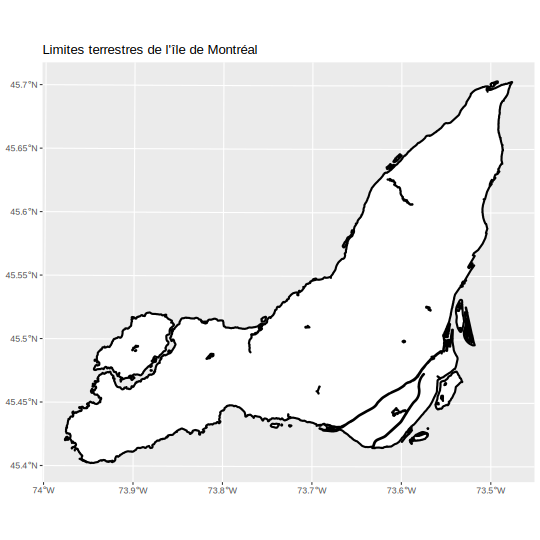
\includegraphics{index_files/figure-latex/plot-terre-1.pdf} La fonction
\texttt{geom\_sf()} permet de faire des représentations simples d'objets
vectoriels de différentes géométries (points, lignes ou polygones).
Cette fonction peut prendre plusieurs arguments\footnote{Pour plus
  d'information sur la fonction \texttt{geom\_sf}, consultez le chapitre
  \href{https://ggplot2.tidyverse.org/reference/ggsf.html}{Visualise sf
  objects} {[}@Wickham\_ggplot2\_2016{]}}. Les arguments utilisés ici
sont les données, la taille du trait avec laquelle on illustre l'objet,
la couleur du trait, et la couleur de la surface délimitée par le trait.
La fonction ggtitle permet d'ajouter un titre à la figure générée.
Remarquez que chaque fonction est écrite sur sa propre ligne, pour
faciliter la lecture des lignes de commande, et que chaque fonction qui
s'ajoute à \texttt{ggplot()} est précédée par le signe plus \texttt{+}.

Dans un deuxième temps, visualisons les pistes cyclables (Fig
@ref(fig:plot-velo)).

\begin{Shaded}
\begin{Highlighting}[]
\KeywordTok{ggplot}\NormalTok{() }\OperatorTok{+}
\KeywordTok{geom_sf}\NormalTok{(}\DataTypeTok{data =}\NormalTok{ pistes_cyclables, }\DataTypeTok{size =} \DecValTok{1}\NormalTok{, }\DataTypeTok{color =} \StringTok{"darkgreen"}\NormalTok{) }\OperatorTok{+}
\KeywordTok{ggtitle}\NormalTok{(}\StringTok{"Pistes cyclables sur l'île de Montréal"}\NormalTok{)}
\end{Highlighting}
\end{Shaded}

\begin{figure}
\centering
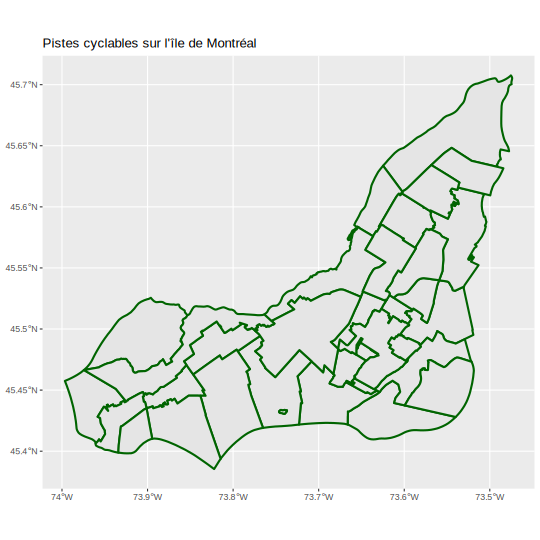
\includegraphics{index_files/figure-latex/plot-velo-1.pdf}
\caption{Pistes cyclables sur l'île de Montréal}
\end{figure}

Pour visualiser des lignes, nous n'avons pas besoin de définir
l'argument \texttt{fill}. Vous remarquerez que les lignes, cette fois,
sont vertes foncées (\texttt{darkgreen}).

Il existe 657 couleurs prédéfinies dans \texttt{R}. Taper la commande
\texttt{colors()} dans votre console \texttt{R} pour voir afficher le
nom des couleurs. Celles-sont sont listées par ordre alphabétique sauf
pour la première couleur, qui est le blanc (\texttt{white}). Ainsi, vous
pouvez utiliser une couleur en assignant son nom ou son numéro. Pour
produire la figure précédente, \texttt{color\ =\ "darkgreen"} aurait pu
être remplacé par \texttt{color\ =\ colors(){[}81{]}}. Essayez pour
voir.

Les couleurs peuvent aussi être définies selon leur composition en
rouge, vert et bleu sur un intervalle allant de 0 à 255 - ce qu'on nomme
le vecteur RGB (red, green, blue). Par exemple, la couleur jaune est
représentée par le vecteur RGB (255, 255, 0). La couleur verte foncée,
utilisée précédemment, est, quant à elle, représentée par le vecteur RGB
(0, 100, 0). Les couleurs peuvent aussi être exprimée selon le système
de notation
\href{https://fr.wikipedia.org/wiki/Syst\%C3\%A8me_hexad\%C3\%A9cimal}{hexadécimal}.
La fonction `rgb' permet de traduire un vecteur de couleur RGB en
notation hexadécimal. Ainsi, pour produire la figure précédente, nous
aurions définir le vecteur
\texttt{vert\_fonce\ =\ rgb(0,\ 100,\ 0,\ maxColorValue=255)}, et
remplacé \texttt{color\ =\ "darkgreen"} par
\texttt{color\ =\ vert\_fonce}. Essayez pour voir.

Pour en apprendre davantage sur les couleurs dans \texttt{R}, vous êtes
invité à consulter le site
\href{https://github.com/EarlGlynn/colorchart/wiki/Color-Chart-in-R}{Earl
Glynn} et à conserver dans vos notes son
\href{Module3/3_TableauCouleurs.pdf}{tableau synthèse des couleurs} dans
\texttt{R}.

Finalement, visualisons les accidents de la route impliquant des
bicyclettes (Fig @ref(fig:plot-accidents)).

\begin{Shaded}
\begin{Highlighting}[]
\KeywordTok{ggplot}\NormalTok{() }\OperatorTok{+}
\KeywordTok{geom_sf}\NormalTok{(}\DataTypeTok{data =}\NormalTok{ accidents_velo, }\DataTypeTok{pch =} \DecValTok{19}\NormalTok{, }\DataTypeTok{cex =} \FloatTok{1.25}\NormalTok{, }\DataTypeTok{color =} \StringTok{"red"}\NormalTok{) }\OperatorTok{+}
\KeywordTok{ggtitle}\NormalTok{(}\StringTok{"Accidents de la route avec cyclistes sur l'île de Montréal"}\NormalTok{)}
\end{Highlighting}
\end{Shaded}

\begin{figure}
\centering
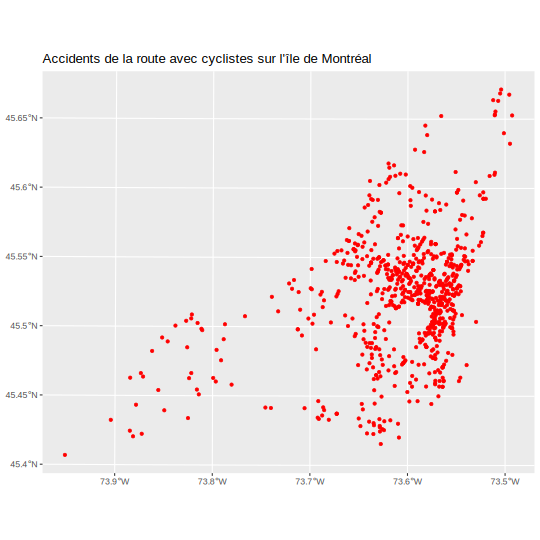
\includegraphics{index_files/figure-latex/plot-accidents-1.pdf}
\caption{Accidents de la route avec cyclistes sur l'île de Montréal}
\end{figure}

Le symbole utilisé pour illustrer la position des accidents est défini
par l'argument \texttt{pch\ =\ 19}. Il existe 25 formats de points
différents prédéfinis dans \texttt{R}. Les voici:

\begin{figure}
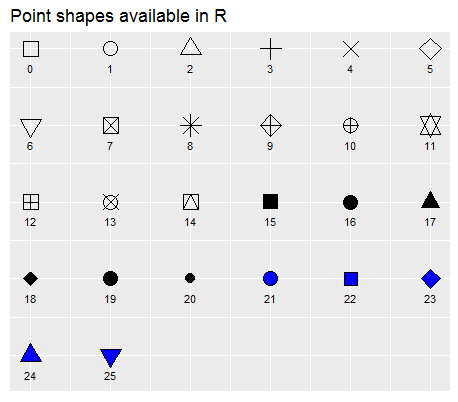
\includegraphics[width=0.5\linewidth]{Module3/3_symbolesR} \caption{Symboles disponibles}\label{fig:plot-symbols}
\end{figure}

L'argument \texttt{cex}, quant à lui, indique le facteur par lequel la
taille du symbole sera augmentée ou réduite par rapport à 1, la valeur
par défaut. Par exemple, `cex = 1.5' indique que le symbole sera 50\%
plus grand, alors que 0.5 indique que le symbole sera 50\% plus petit.

Ainsi, nous pouvons changer les valeurs de ces arguments et représenter
les accidents de vélo par des triangles oranges (Fig
@ref(fig:plot-accidents2)).

\begin{Shaded}
\begin{Highlighting}[]
\KeywordTok{ggplot}\NormalTok{() }\OperatorTok{+}
\KeywordTok{geom_sf}\NormalTok{(}\DataTypeTok{data =}\NormalTok{ accidents_velo, }\DataTypeTok{pch =} \DecValTok{24}\NormalTok{, }\DataTypeTok{cex =} \FloatTok{1.5}\NormalTok{, }\DataTypeTok{color =} \StringTok{"black"}\NormalTok{, }\DataTypeTok{fill =} \StringTok{"orange"}\NormalTok{) }\OperatorTok{+}
\KeywordTok{ggtitle}\NormalTok{(}\StringTok{"Accidents de la route avec cyclistes sur l'île de Montréal"}\NormalTok{)}
\end{Highlighting}
\end{Shaded}

\begin{figure}
\centering
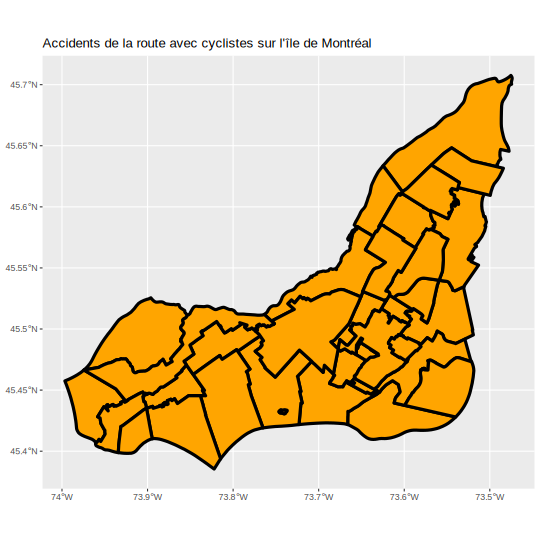
\includegraphics{index_files/figure-latex/plot-accidents2-1.pdf}
\caption{Symbole et couleur différents pour illustrer les accidents de
la route avec cyclistes sur l'île de Montréal}
\end{figure}

\paragraph{Visualiser des données vectorielles par
attribut}\label{visualiser-des-donnuxe9es-vectorielles-par-attribut}
\addcontentsline{toc}{paragraph}{Visualiser des données vectorielles par
attribut}

Lorsque nous avons affiché les métadonnées du shapefile
\texttt{pistes\_cyclables}, vous avez peut-être observé que ce dernier
comprenait l'attribut \texttt{TYPE\_VOIE} qui caractérise le type de
pistes cyclables de chaque multiligne. Affichez les métadonnées à
nouveau:

\begin{Shaded}
\begin{Highlighting}[]
\NormalTok{pistes_cyclables}
\end{Highlighting}
\end{Shaded}

\begin{verbatim}
## Simple feature collection with 34 features and 10 fields
## geometry type:  MULTIPOLYGON
## dimension:      XY
## bbox:           xmin: -73.9966 ymin: 45.3854 xmax: -73.47387 ymax: 45.70758
## epsg (SRID):    4326
## proj4string:    +proj=longlat +datum=WGS84 +no_defs
## First 10 features:
##    MUNID CODEID CODEMAMROT                                      NOM
## 1  66023     11      REM05                                Outremont
## 2  66023     22      REM17                                  LaSalle
## 3  66023     62      66072                               Mont-Royal
## 4  66023      9      REM19                              Ville-Marie
## 5  66023      5      REM21                    Le Plateau-Mont-Royal
## 6  66023     54      66062                                Hampstead
## 7  66023     63      REM20                             Le Sud-Ouest
## 8  66023     57      REM33 Rivière-des-Prairies-Pointe-aux-Trembles
## 9  66023     28      REM27                                  Lachine
## 10 66023     51      66087                                   Dorval
##              TYPE ABREV NUM     AIRE     PERIM                       geometry
## 1  Arrondissement    OM   5  3813356 10836.670 MULTIPOLYGON (((-73.62078 4...
## 2  Arrondissement    LS  18 25197268 25259.849 MULTIPOLYGON (((-73.6661 45...
## 3      Ville liée    MR   2  7445560 18314.038 MULTIPOLYGON (((-73.65075 4...
## 4  Arrondissement    VM  20 21500632 26585.959 MULTIPOLYGON (((-73.53013 4...
## 5  Arrondissement    PM  22  8151665 13158.328 MULTIPOLYGON (((-73.55923 4...
## 6      Ville liée    HS  10  1768055  5875.848 MULTIPOLYGON (((-73.65601 4...
## 7  Arrondissement    SO  21 18144269 29633.161 MULTIPOLYGON (((-73.62908 4...
## 8  Arrondissement    RP  19 50047004 38573.067 MULTIPOLYGON (((-73.62475 4...
## 9  Arrondissement    LC  17 23127786 25399.526 MULTIPOLYGON (((-73.72299 4...
## 10     Ville liée    DV   1 28156150 32357.566 MULTIPOLYGON (((-73.7947 45...
##    TYPE_VOIE
## 1          1
## 2          2
## 3          3
## 4          4
## 5          5
## 6          1
## 7          2
## 8          3
## 9          4
## 10         5
\end{verbatim}

Utilisons la fonction \texttt{levels} pour connaître ces types de voie
cyclables. La fonction \texttt{levels} donne les différentes valeurs que
peuvent prendre un attribut.

\begin{Shaded}
\begin{Highlighting}[]
\KeywordTok{levels}\NormalTok{(pistes_cyclables}\OperatorTok{$}\NormalTok{TYPE_VOIE)}
\end{Highlighting}
\end{Shaded}

\begin{verbatim}
## NULL
\end{verbatim}

Si vous ne connaissez pas la distinction entre ces types d'aménagement
cyclable, consulter ce
\href{Module3/3_Amenagement3Cyclable3Mtl.pdf}{document sommaire} de la
\emph{Ville de Montréal}\footnote{Ville de Montréal. Aménagements
  cyclables. Repéré le 19 mars 2020}

Nous voulons maintenant représenter les données vectorielles associées
aux pistes cyclables de type \texttt{"Bande\ cyclable"}. Pour
représenter une valeur précise d'un attribut, nous utiliserons la
fonction \texttt{filter} de la librarie \texttt{dplyr}. Commençons par
charger cette librairie.

\begin{Shaded}
\begin{Highlighting}[]
\KeywordTok{library}\NormalTok{(dplyr)}
\end{Highlighting}
\end{Shaded}

Utilisons la fonction \texttt{filter} qui permet de filtrer l'ensemble
des valeurs de l'attribut \texttt{TYPE\_VOIE}, pour ne retenir que les
données dont la valeur est identique (ce qui s'exprime par l'opération
\texttt{==}) à `\,``Bande cyclable''\,'. Nous nommerons ce sous-ensemble
de données \texttt{Bande}.

\begin{Shaded}
\begin{Highlighting}[]
\NormalTok{Bande <-pistes_cyclables }\OperatorTok
\StringTok{  }\KeywordTok{filter}\NormalTok{(TYPE_VOIE }\OperatorTok{==}\StringTok{"Bande cyclable"}\NormalTok{)}
\end{Highlighting}
\end{Shaded}

Nous représentons ce sous-ensemble de données de la même manière que
pour l'ensemble complet (Fig @ref(fig:plot-velo)).

\begin{Shaded}
\begin{Highlighting}[]
\KeywordTok{ggplot}\NormalTok{()}\OperatorTok{+}
\StringTok{  }\KeywordTok{geom_sf}\NormalTok{(}\DataTypeTok{data =}\NormalTok{ Bande,  }\DataTypeTok{size =} \DecValTok{1}\NormalTok{, }\DataTypeTok{color =} \StringTok{"darkgreen"}\NormalTok{)}\OperatorTok{+}
\StringTok{  }\KeywordTok{ggtitle}\NormalTok{(}\StringTok{"Pistes cyclables sur l'île de Montréal"}\NormalTok{, }\DataTypeTok{subtitle =} \StringTok{"Bande cyclable"}\NormalTok{)}
\end{Highlighting}
\end{Shaded}

\begin{figure}
\centering
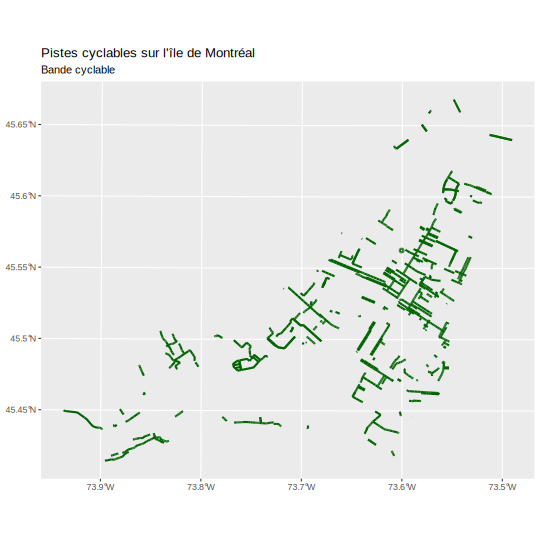
\includegraphics{index_files/figure-latex/plot-voie3-1.pdf}
\caption{Bandes cyclables sur l'île de Montréal}
\end{figure}

Nous voulons maintenant représenter les six types de voie cyclable par
six couleurs différentes. Créons d'abord un vecteur de six couleurs,
qu'on appelle une palette de couleurs.

\begin{Shaded}
\begin{Highlighting}[]
\NormalTok{couleurs_voie<-}\KeywordTok{c}\NormalTok{(}\StringTok{"darkgreen"}\NormalTok{, }\StringTok{"turquoise"}\NormalTok{, }\StringTok{"yellow"}\NormalTok{,}\StringTok{"darkblue"}\NormalTok{,}\StringTok{"violet"}\NormalTok{,}\StringTok{"orange"}\NormalTok{)}
\end{Highlighting}
\end{Shaded}

Nous pouvons demander à \texttt{ggplot} d'utiliser ces couleurs pour
illustrer les différents types de voie cyclable (Fig
@ref(fig:plot-voie5)).

\begin{Shaded}
\begin{Highlighting}[]
\KeywordTok{ggplot}\NormalTok{()}\OperatorTok{+}
\StringTok{  }\CommentTok{# geom_sf(data = pistes_cyclables,  aes(color = TYPE_VOIE))+}
\StringTok{  }\KeywordTok{scale_color_manual}\NormalTok{(}\DataTypeTok{values =}\NormalTok{ couleurs_voie)}\OperatorTok{+}
\StringTok{  }\KeywordTok{labs}\NormalTok{(}\DataTypeTok{color =} \StringTok{'Types de voie'}\NormalTok{)}\OperatorTok{+}
\StringTok{  }\KeywordTok{ggtitle}\NormalTok{(}\StringTok{"Pistes cyclables sur l'île de Montréal"}\NormalTok{, }\DataTypeTok{subtitle =} \StringTok{"Types de voie"}\NormalTok{)}
\end{Highlighting}
\end{Shaded}

\begin{figure}
\centering
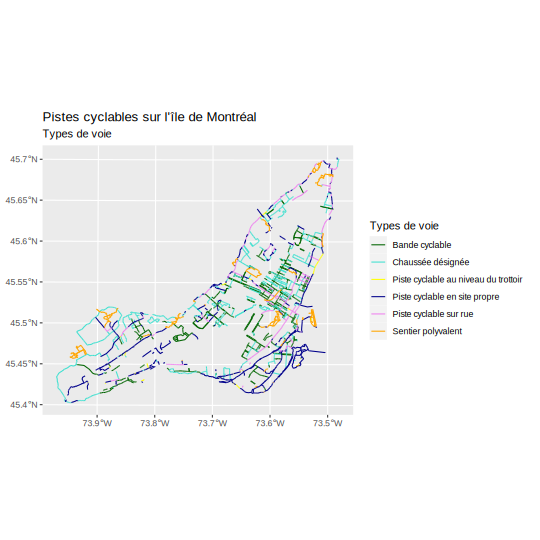
\includegraphics{index_files/figure-latex/plot-voie5-1.pdf}
\caption{Types de voie cyclable sur l'île de Montréal}
\end{figure}

La fonction \texttt{aes} décrit quelles variables dans les données
(\texttt{data}) sont illustrées (dans notre exemple, ce sont
\texttt{TYPE\_VOIE}) et par quelles caractéristiques visuelles\footnote{Pour
  plus d'information sur la fonction \texttt{aes}, consultez le chapitre
  \href{https://ggplot2.tidyverse.org/reference/aes.html}{Construct
  aesthetic mappings} {[}@Wickham\_ggplot2\_2016{]}}. On nomme ces
caractéristiques visuelles les ``esthétiques'' (\texttt{aes} pour
``aesthetic'' en anglais). Dans le présent exemple, nous nous
préoccupons seulement de la couleur des données vectorielles, mais nous
aurions pu aussi changer leur taille, le type de lignes, ou la forme des
symboles (si la géométrie des données étaient de type point).

La fonction \texttt{scale\_color\_manual} permet de spécifier nos
propres couleurs, sans quoi ce seront les couleurs par défaut qui seront
utilisées\footnote{Pour plus d'information sur la fonction
  \texttt{scale\_colour\_manual}, consultez le chapitre
  \href{https://ggplot2.tidyverse.org/reference/scale_manual.html}{Create
  your own discrete scale} {[}@Wickham\_ggplot2\_2016{]}}.

Finalement, la fonction \texttt{labs} permet d'assigner un titre à la
légende, sans quoi c'est le nom de la variable, telle que nous l'avons
définie dans \texttt{R} qui sera affichée, ici, \texttt{TYPE\_VOIE}.

Nous pouvons aussi demander à \texttt{ggplot} de représenter les types
de voie cyclable en utilisant différentes tailles de trait. De la même
façon que précédemment, nous créons un vecteur de six tailles.

\begin{Shaded}
\begin{Highlighting}[]
\NormalTok{tailles_voie<-}\KeywordTok{c}\NormalTok{(}\DecValTok{1}\NormalTok{,}\FloatTok{1.2}\NormalTok{,}\FloatTok{1.5}\NormalTok{,}\FloatTok{1.7}\NormalTok{,}\DecValTok{2}\NormalTok{,}\FloatTok{2.2}\NormalTok{)}
\end{Highlighting}
\end{Shaded}

Puis représentatons les types de voie cyclable (Fig
@ref(fig:plot-voie7)).

\begin{Shaded}
\begin{Highlighting}[]
\KeywordTok{ggplot}\NormalTok{()}\OperatorTok{+}
\StringTok{  }\CommentTok{# geom_sf(data = pistes_cyclables,  aes(color = TYPE_VOIE, size = TYPE_VOIE))+}
\StringTok{  }\KeywordTok{scale_color_manual}\NormalTok{(}\DataTypeTok{values =}\NormalTok{ couleurs_voie)}\OperatorTok{+}
\StringTok{  }\KeywordTok{labs}\NormalTok{(}\DataTypeTok{color =} \StringTok{'Types de voie'}\NormalTok{)}\OperatorTok{+}
\StringTok{  }\KeywordTok{scale_size_manual}\NormalTok{(}\DataTypeTok{values =}\NormalTok{ tailles_voie)}\OperatorTok{+}
\StringTok{  }\KeywordTok{labs}\NormalTok{(}\DataTypeTok{size =} \StringTok{'Types de voie'}\NormalTok{)}\OperatorTok{+}
\StringTok{  }\KeywordTok{ggtitle}\NormalTok{(}\StringTok{"Pistes cyclables sur l'île de Montréal"}\NormalTok{, }\DataTypeTok{subtitle =} \StringTok{"Types de voie"}\NormalTok{)}\OperatorTok{+}
\StringTok{  }\KeywordTok{theme}\NormalTok{(}\DataTypeTok{legend.position =} \StringTok{"bottom"}\NormalTok{)}
\end{Highlighting}
\end{Shaded}

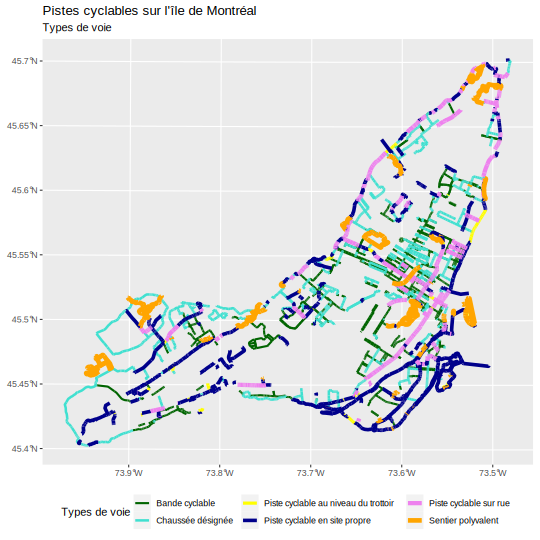
\includegraphics{index_files/figure-latex/plot-voie7-1.pdf} La légende
tient compte à la fois de la couleur, et de la taille des traits. De
plus, nous l'avons affichée au bas de la figure.

\paragraph{Visualiser plusieurs
shapefiles}\label{visualiser-plusieurs-shapefiles}
\addcontentsline{toc}{paragraph}{Visualiser plusieurs shapefiles}

Nous allons maintenant représenter les données vectorielles
\texttt{limites\ terrestres}, \texttt{pistes\_cyclables} et
\texttt{accidents\_velo} au sein d'une même figure. Il s'agit d'utiliser
la fonction \texttt{geom\_sf} pour chaque couche de données et de les
combiner en utilisant le \texttt{+}.

\begin{Shaded}
\begin{Highlighting}[]
\KeywordTok{ggplot}\NormalTok{()}\OperatorTok{+}
\StringTok{  }\KeywordTok{geom_sf}\NormalTok{(}\DataTypeTok{data =}\NormalTok{ limites_terrestres, }\DataTypeTok{size =} \DecValTok{1}\NormalTok{, }\DataTypeTok{color =} \StringTok{"black"}\NormalTok{, }\DataTypeTok{fill =} \StringTok{"white"}\NormalTok{)}\OperatorTok{+}
\StringTok{  }\KeywordTok{geom_sf}\NormalTok{(}\DataTypeTok{data =}\NormalTok{ pistes_cyclables, }\DataTypeTok{size =} \DecValTok{1}\NormalTok{, }\DataTypeTok{color =} \StringTok{"darkgreen"}\NormalTok{)}\OperatorTok{+}
\StringTok{  }\KeywordTok{geom_sf}\NormalTok{(}\DataTypeTok{data =}\NormalTok{ accidents_velo, }\DataTypeTok{pch =} \DecValTok{19}\NormalTok{, }\DataTypeTok{cex =} \FloatTok{1.25}\NormalTok{, }\DataTypeTok{color =} \StringTok{"red"}\NormalTok{)}\OperatorTok{+}
\StringTok{  }\KeywordTok{ggtitle}\NormalTok{(}\StringTok{"Pistes cyclables sur l'île de Montréal et Accidents routiers impliquant des vélos"}\NormalTok{)}
\end{Highlighting}
\end{Shaded}

\begin{figure}
\centering
\includegraphics{index_files/figure-latex/plot-all1-1.pdf}
\caption{Pistes cyclables et position des accidents routiers impliquant
des bicyclettes sur l'île de Montréal}
\end{figure}

Nous pouvons créer une carte plus précise qui spécifie les types de voie
cyclable et ajouter une légende.

\begin{Shaded}
\begin{Highlighting}[]
\KeywordTok{ggplot}\NormalTok{()}\OperatorTok{+}
\StringTok{  }\KeywordTok{geom_sf}\NormalTok{(}\DataTypeTok{data =}\NormalTok{ limites_terrestres, }\DataTypeTok{size =} \DecValTok{1}\NormalTok{, }\DataTypeTok{color =} \StringTok{"black"}\NormalTok{, }\DataTypeTok{fill =} \StringTok{"white"}\NormalTok{)}\OperatorTok{+}
\StringTok{  }\CommentTok{# geom_sf(data = pistes_cyclables, size = 1.5, aes(color = TYPE_VOIE),  show.legend = "line")+}
\StringTok{  }\KeywordTok{scale_color_manual}\NormalTok{(}\DataTypeTok{values =}\NormalTok{ couleurs_voie,}\DataTypeTok{name =} \StringTok{"Types de voie"}\NormalTok{)}\OperatorTok{+}
\StringTok{  }\KeywordTok{geom_sf}\NormalTok{(}\DataTypeTok{data =}\NormalTok{ accidents_velo, }\DataTypeTok{pch =} \DecValTok{24}\NormalTok{, }\DataTypeTok{cex =} \DecValTok{2}\NormalTok{, }\DataTypeTok{fill =} \StringTok{"red"}\NormalTok{, }\DataTypeTok{color =} \StringTok{"black"}\NormalTok{)}\OperatorTok{+}
\StringTok{  }\KeywordTok{ggtitle}\NormalTok{(}\StringTok{"Types de voie cyclable et Accidents routiers impliquant des vélos"}\NormalTok{)}\OperatorTok{+}
\KeywordTok{theme}\NormalTok{(}
      \CommentTok{#Caractéristiques de la figure elle-même}
      \DataTypeTok{panel.background =} \KeywordTok{element_rect}\NormalTok{(}\DataTypeTok{fill =} \StringTok{"black"}\NormalTok{), }\CommentTok{#le dessous de la carte}
      \DataTypeTok{plot.background =} \KeywordTok{element_rect}\NormalTok{(}\DataTypeTok{fill =} \StringTok{"black"}\NormalTok{),  }\CommentTok{#le contour de la carte}
      \DataTypeTok{panel.grid.major =} \KeywordTok{element_blank}\NormalTok{(),              }\CommentTok{#retirer la grille cartésienne}
      \DataTypeTok{axis.ticks =} \KeywordTok{element_blank}\NormalTok{(),                    }\CommentTok{#retirer les traits sur les axes}
      \DataTypeTok{axis.text.x =} \KeywordTok{element_blank}\NormalTok{(),                   }\CommentTok{#retirer les traits les noms ou les numéros de ces traits}
      \DataTypeTok{axis.text.y =} \KeywordTok{element_blank}\NormalTok{(),}
      \DataTypeTok{plot.title =} \KeywordTok{element_text}\NormalTok{(}\DataTypeTok{colour =} \StringTok{"white"}\NormalTok{, }\DataTypeTok{size =} \DecValTok{16}\NormalTok{, }\DataTypeTok{hjust =} \FloatTok{0.5}\NormalTok{), }\CommentTok{#Centrer le titre de la carte}
      \CommentTok{#Caractéristiques de la légende}
      \DataTypeTok{legend.position =} \StringTok{"top"}\NormalTok{,                         }\CommentTok{#position de la légende}
      \DataTypeTok{legend.title =} \KeywordTok{element_text}\NormalTok{(}\DataTypeTok{colour=}\StringTok{"blue"}\NormalTok{, }\DataTypeTok{size =} \DecValTok{11}\NormalTok{, }\DataTypeTok{face =} \StringTok{"bold"}\NormalTok{), }\CommentTok{#titre de la légende}
      \DataTypeTok{legend.text =} \KeywordTok{element_text}\NormalTok{(}\DataTypeTok{size =} \DecValTok{10}\NormalTok{, }\DataTypeTok{face =} \StringTok{"italic"}\NormalTok{),               }\CommentTok{#texte des éléments de la légende}
      \DataTypeTok{legend.background =} \KeywordTok{element_rect}\NormalTok{(}\DataTypeTok{fill =} \StringTok{"white"}\NormalTok{, }\DataTypeTok{size =} \DecValTok{1}\NormalTok{, }\DataTypeTok{linetype =} \StringTok{"solid"}\NormalTok{, }\DataTypeTok{colour =} \StringTok{"red"}\NormalTok{), }\CommentTok{#rectangle autour de la légende}
      \DataTypeTok{legend.key =} \KeywordTok{element_rect}\NormalTok{(}\DataTypeTok{fill =} \StringTok{"white"}\NormalTok{)        }\CommentTok{#couleur blanche sous les éléments de la légende}
\NormalTok{)}
\end{Highlighting}
\end{Shaded}

\includegraphics{index_files/figure-latex/plot-all2-1.pdf} La fonction
\texttt{theme()} permet de d'ajuster l'apparence de la carte (couleur du
fond, couleur, taille et position du titre, format de la légende, etc.).
Le chapitre
\href{https://ggplot2.tidyverse.org/reference/theme.html}{Modify
components of theme} {[}@Wickham\_ggplot2\_2016{]} énumère l'ensemble
des paramètres pouvant être modifiés pour changer l'apparence d'une
carte.

\subsubsection{Reprojection de données vectorielles sous
R}\label{reprojection-de-donnuxe9es-vectorielles-sous-r}

Dans cette section nous apprendrons à manipuler le système de
coordonnées de référence de données vectorielles. Nous avons vu en début
de leçon que les données utilisées sont dans la projection de Mercator
transverse (\texttt{tmerc}) et utilisent le Système de référence
géodésique nord-américan de 1983 (\texttt{NAD83}). Par exemple, pour
connaître le SCR des données \texttt{limites\_terrestres} nous avions
fait.

\begin{Shaded}
\begin{Highlighting}[]
\KeywordTok{st_crs}\NormalTok{(limites_terrestres)}
\end{Highlighting}
\end{Shaded}

\begin{verbatim}
## Coordinate Reference System:
##   No EPSG code
##   proj4string: "+proj=tmerc +lat_0=0 +lon_0=-73.5 +k=0.9999 +x_0=304800 +y_0=0 +datum=NAD83 +units=m +no_defs"
\end{verbatim}

Nous allons maintenant transformer le SCR vers la projection de Robinson
(\texttt{robin}) et le Système géodésique mondial de 1984
(\texttt{WGS84}). Pour se faire nous utilisons la fonction
\texttt{st\_transform} de la librarie \texttt{st}.

\begin{Shaded}
\begin{Highlighting}[]
\NormalTok{limites_terrestres_rob <-}\StringTok{ }\KeywordTok{st_transform}\NormalTok{(limites_terrestres,}
    \KeywordTok{CRS}\NormalTok{(}\StringTok{"+proj=robin +datum=WGS84"}\NormalTok{))}
\end{Highlighting}
\end{Shaded}

Comparons les données transformées avec les données initiales. Pour se
faire, nous voulons représenter les deux cartes une au-dessous de
l'autre. La librarie \texttt{ggpubr} permet de créer facilement des
figures avec des panneaux multiples. Installez la librarie si ce n'est
pas déjà fait, et chargez-là dans votre session de travail.

\begin{Shaded}
\begin{Highlighting}[]
\KeywordTok{library}\NormalTok{(ggpubr)}
\end{Highlighting}
\end{Shaded}

\begin{Shaded}
\begin{Highlighting}[]
\NormalTok{carte1<-}\KeywordTok{ggplot}\NormalTok{()}\OperatorTok{+}
\StringTok{  }\KeywordTok{geom_sf}\NormalTok{(}\DataTypeTok{data =}\NormalTok{ limites_terrestres, }\DataTypeTok{size =} \DecValTok{1}\NormalTok{, }\DataTypeTok{color =} \StringTok{"black"}\NormalTok{, }\DataTypeTok{fill =} \StringTok{"white"}\NormalTok{) }\OperatorTok{+}
\StringTok{  }\KeywordTok{ggtitle}\NormalTok{(}\StringTok{"Projection Mercator"}\NormalTok{)}
\NormalTok{carte2<-}\KeywordTok{ggplot}\NormalTok{()}\OperatorTok{+}
\StringTok{  }\KeywordTok{geom_sf}\NormalTok{(}\DataTypeTok{data =}\NormalTok{ limites_terrestres_rob, }\DataTypeTok{size =} \DecValTok{1}\NormalTok{, }\DataTypeTok{color =} \StringTok{"black"}\NormalTok{, }\DataTypeTok{fill =} \StringTok{"yellow"}\NormalTok{) }\OperatorTok{+}
\StringTok{  }\KeywordTok{ggtitle}\NormalTok{(}\StringTok{"Projection Robinson"}\NormalTok{)}
\NormalTok{figure <-}\StringTok{ }\KeywordTok{ggarrange}\NormalTok{(carte1, carte2, }\DataTypeTok{labels =} \KeywordTok{c}\NormalTok{(}\StringTok{"A"}\NormalTok{,}\StringTok{"B"}\NormalTok{),}\DataTypeTok{ncol =} \DecValTok{1}\NormalTok{, }\DataTypeTok{nrow =} \DecValTok{2}\NormalTok{)}
\NormalTok{figure}
\end{Highlighting}
\end{Shaded}

\begin{figure}
\centering
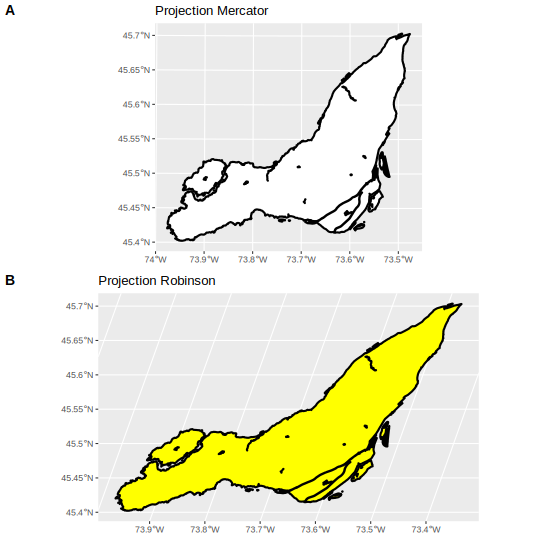
\includegraphics{index_files/figure-latex/plot-terre2-1.pdf}
\caption{Limites terrestres de l'île de Montréal selon les projections
Mercartor (A) et Robinson (B)}
\end{figure}

Finalement, pour sauvegarder des données vectorielles, nous utilisons la
fonction \texttt{st\_write} de la librarie \texttt{st}, de la même façon
que nous avons utilisé la fonction \texttt{st\_read} en début de leçon.
Par exemple, sauvons les données \texttt{limites\_terrestres\_rob} que
nous venons de créer.

\begin{Shaded}
\begin{Highlighting}[]
\NormalTok{chemin<-}\StringTok{"D:/votrechemin/SCI1031/Module3/Donnees/"}
\NormalTok{nom_du_fichier<-}\StringTok{ }\KeywordTok{paste}\NormalTok{(chemin, }\StringTok{"/Montreal_Velo/terre/terre_rob_shp.shp"}\NormalTok{, }\DataTypeTok{sep =} \StringTok{""}\NormalTok{)}
\KeywordTok{st_read}\NormalTok{(limites_terrestres_rob,nom_du_fichier)}
\end{Highlighting}
\end{Shaded}

\subsection{Exercice}\label{exercice}

\end{document}
